\let\negmedspace\undefined
\let\negthickspace\undefined
\documentclass[journal]{IEEEtran}
\usepackage[a5paper, margin=10mm, onecolumn]{geometry}
\usepackage{lmodern} % Ensure lmodern is loaded for pdflatex
 % Include tfrupee package
\setlength{\headheight}{1cm} % Set the height of the header box
\setlength{\headsep}{0mm}     % Set the distance between the header box and the top of the text
\usepackage{enumitem}
\usepackage{gvv-book}
\usepackage{gvv}
\usepackage{cite}
\usepackage{amsmath,amssymb,amsfonts,amsthm}
\usepackage{algorithmic}
\usepackage{graphicx}
\usepackage{textcomp}
\usepackage{xcolor}
\usepackage{txfonts}
\usepackage{listings}
\usepackage{enumitem}
\usepackage{mathtools}
\usepackage{gensymb}
\usepackage{graphicx}
\usepackage{wrapfig}
\usepackage{comment}
\usepackage[breaklinks=true]{hyperref}
\usepackage{tkz-euclide} 
\usepackage{listings}
% \usepackage{gvv}                                        
\def\inputGnumericTable{}                                 
\usepackage[latin1]{inputenc}                                
\usepackage{color}                                            
\usepackage{array}                                            
\usepackage{longtable}                                       
\usepackage{calc}                                             
\usepackage{multirow}                                         
\usepackage{hhline}                                           
\usepackage{ifthen}                                           
\usepackage{lscape}
\begin{document}

\bibliographystyle{IEEEtran}
\vspace{3cm}


\author{AI24BTECH11008- Sarvajith
}
\title{Assignment 7}
% \maketitle
% \newpage
% \bigskip
{\let\newpage\relax\maketitle}
\title{2007, CE}
\renewcommand{\thefigure}{\theenumi}
\renewcommand{\thetable}{\theenumi}
\setlength{\intextsep}{10pt} % Space between text and floats
\numberwithin{equation}{enumi}
\numberwithin{figure}{enumi}
\renewcommand{\thetable}{\theenumi}
\begin{enumerate}
  \item[35.]The right triangular truss is made of members having equal cross sectional area of
  $1550 mm^2$ and Young's modulus of $2 x 10^5$ MPa. The horizontal deflection of the
  joint $Q$ is 
  \begin{figure}[!ht]
    \centering
    
    \resizebox{0.3\textwidth}{!}{%
    \begin{circuitikz}
    \tikzstyle{every node}=[font=\normalsize]
    \draw [short] (3.75,10.25) -- (3.75,7.75);
    \draw [short] (3.75,7.75) -- (7.25,7.75);
    \draw [short] (4,8.75) -- (7,8.75);
    \node [font=\normalsize] at (7.25,7.5) {B};
    \node [font=\normalsize] at (3.25,10) {$\rho_{xy}$};
    \end{circuitikz}
    }%
    
    % Specify the path to your TikZ file
    \caption{ 1}
    \label{fig:triangle_diagram}
\end{figure}
  \begin{enumerate}
    \item [A.] 2.47mm
    \item [B.] 10.25mm
    \item [C.] 14.10mm
    \item [D.] 15.68mm
  \end{enumerate}
  \item[36.] The influence line diagram (ILD) shown is for the member
  \begin{figure}[h!]
    \centering
    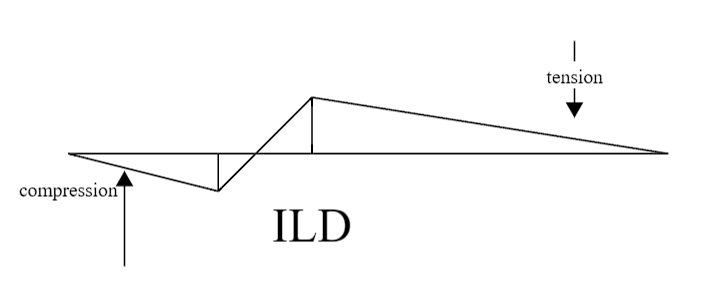
\includegraphics[width=0.3\textwidth]{figs/image.png}  % Replace with your image file
    
    \label{fig:sample2}
\end{figure}
 \begin{figure}[h!]
 \centering
 
    \resizebox{0.3\textwidth}{!}{%
    \begin{circuitikz}
    \tikzstyle{every node}=[font=\normalsize]
    
    \draw (-5.5,13.25) to[R] (-3.5,13.25);
    \draw (-2,13.75) node[op amp,scale=1, yscale=-1 ] (opamp2) {};
    \draw (opamp2.+) to[short] (-3.5,14.25);
    \draw  (opamp2.-) to[short] (-3.5,13.25);
    \draw (-0.8,13.75) to[short](-0.5,13.75);
    \draw (-3.5,14.25) to (-4,14.25) node[ground]{};
    \draw [short] (-3,13.25) -- (-3,12.25);
    \draw [short] (-1,13.75) -- (-1,12.25);
    \draw (-3,12.25) to[empty Schottky diode] (-1,12.25);
    \node [font=\normalsize] at (-2,11.75) {5.1V};
    \end{circuitikz}
    }%
    
   
 \label{fig:sample1}
 \end{figure}
    
    \begin{enumerate}
        \item [A.] PS
        \item [B.] RS
        \item [C.] PQ
        \item [D.] QS
    \end{enumerate}
  \item[37.]  Consider the following statements: 
  \begin{enumerate}
    \item The compressive strength of concrete decreases with increase in watercement ratio of the concrete mix.
    \item Water is added to the concrete mix for hydration of cement and
    workability. 
    \item Creep and shrinkage of concrete are independent of the water-cement ratio
    in the concrete mix
  \end{enumerate}
  The true statements are 
  \begin{enumerate}
    \item [A.] a and b
    \item [B.] a,b and c
    \item [C.] b and c
    \item [D.] only b
  \end{enumerate}
  \item [38.] The percentage loss of prestress due to anchorage slip of 3mm in a concrete beam
  of length $30m$ which is post-tensioned by a tendon with an initial stress of 1200 $\frac{N}{mm^2}$
  and modulus of elasticity equal to $2.1 x 10^5\frac{N}{mm^2}$ is
  \begin{enumerate}
    \item [A.] 0.0175 
    \item [B.] 0.175 
    \item [C.] 1.75 
    \item [D.] 17.5 
  \end{enumerate}
  \item [39.] A concrete beam of rectangular cross-section of size 120mm \brak{width} and 200mm
  \brak{depth} is prestressed by a straight tendon to an effective force of 150kN at an
  eccentricity of 20mm (below the centroidal axis in the depth direction). The
  stresses at the top and bottom fibres of the section are.
  \begin{enumerate}
    \item [A.] $2.5N/mm^2$ \brak{compression}, $10\frac{N}{mm^2}$ \brak{compression}
    \item [A.] $10N/mm^2$ \brak{tension}, $3.75\frac{N}{mm^2}$
    \item [A.] $3.75N/mm^2$ \brak{tension}, $3.75\frac{N}{mm^2}$ \brak{compression}
    \item [A.] $2.75N/mm^2$ \brak{compression}, $3.75\frac{N}{mm^2}$ \brak{compression}
  \end{enumerate}
  \item[40.] Consider the following statements: 
  \begin{enumerate}
    \item [I] Modulus of elasticity concrete increases with increase in compressive
    strength of concrete
    \item [II] Brittleness of concrete increases with decrease in compressive strength of
    concrete
    \item [III] Shear strength of concrete increases with increase in compressive strength
    of concrete. 
  \end{enumerate}
  The true statements are 
  \begin{enumerate}
    \item [A.] II and III
    \item [B.] I, II and III
    \item [C.] I and II
    \item [D.] I and III
  \end{enumerate}
  \item[41]  A steel flat of rectangular section of size 70 x 6 mm is connected to a gusset plate
  by three bolts each having a shear capacity of 15kN in holes having diameter
  11.5mm. If the allowable tensile stress in the flat is 150MPa, the maximum
  tension that can be applied to the flat is
  \begin{figure}[!ht]
    \centering
    
    \resizebox{0.4\textwidth}{!}{%
    \begin{circuitikz}
    \tikzstyle{every node}=[font=\normalsize]
    
    \draw (6.5,12.25) node[ieeestd not port, anchor=in](port){} (port.out) to[short] (8.25,12.25);
    \draw (port.in) to[short] (6.25,12.25);
    \draw (6.5,11) node[ieeestd not port, anchor=in](port){} (port.out) to[short] (8.25,11);
    \draw (port.in) to[short] (6.25,11);
    \draw (6.5,9.75) node[ieeestd not port, anchor=in](port){} (port.out) to[short] (8.25,9.75);
    \draw (port.in) to[short] (6.25,9.75);
    \draw [short] (8.25,12.25) -- (8.75,12);
    \draw [short] (8.25,11) -- (8.75,11.5);
    \draw [short] (8,9.75) -- (11.5,9.75);
    \draw [short] (10.75,11.75) -- (11.5,11.75);
    \draw [short] (11.5,11.75) -- (13,10.75);
    \draw [short] (11.5,9.75) -- (13,10.25);
    \draw [short] (15,10.5) -- (16,10.5);
    \node [font=\normalsize] at (6,12.25) {P};
    \node [font=\normalsize] at (6,11) {R};
    \node [font=\normalsize] at (6,9.75) {Q};
    \node [font=\normalsize] at (16.5,10.5) {Y};
    \draw (8.75,12) to[short] (9,12);
    \draw (8.75,11.5) to[short] (9,11.5);
    \draw (9,12) node[ieeestd and port, anchor=in 1, scale=0.89](port){} (port.out) to[short] (10.75,11.75);
    \draw (13,10.75) to[short] (13.25,10.75);
    \draw (13,10.25) to[short] (13.25,10.25);
    \draw (13.25,10.75) node[ieeestd or port, anchor=in 1, scale=0.89](port){} (port.out) to[short] (15,10.5);
    \end{circuitikz}
    }%
    
    % Specify the path to your TikZ file
    \caption{3 }
    \label{3 }
  \end{figure}
  \begin{enumerate}
    \item [A.] 43.2kN
    \item [B.] 52.65kN
    \item [C.] 59.5kN
    \item [D.] 63.0kN
  \end{enumerate}
  \item[42.] A bracket connection is made with four bolts of 10mm diameter and supports a
  load of 10kN a an eccentricity of 100mm. the maximum force to be resisted by
  any bolt will be 
  \begin{figure}[!ht]
    \centering
    
    \resizebox{0.3\textwidth}{!}{%
    \begin{circuitikz}
    \tikzstyle{every node}=[font=\normalsize]
    \draw (2.5,9.5) to[R] (4.5,9.5);
    \draw (4.5,9.5) to[R] (7.75,9.5);
    \draw (4.75,9.5) to[R] (4.75,6.25);
    \draw (4.75,9.5) to[R] (6.5,7.75);
    \draw (4.75,6.25) to[R] (6,7.5);
    \draw (7.75,9.5) to[R] (7.75,6.25);
    \draw (7.75,9.5) to[R] (11,9.5);
    \draw (11,9.5) to[R] (11,6.25);
    \draw (4.75,6.25) to[R] (2.5,6.25);
    \draw [short] (6,7.5) .. controls (6.5,7.5) and (6.5,7.5) .. (6.5,8);
    \draw [short] (6.5,8) -- (7.75,9.5);
    \draw [short] (4.75,6.25) -- (6.75,6.25);
    \draw [short] (4.75,6.25) -- (7.75,6.25);
    \draw [short] (6.5,7.75) -- (7.75,6.25);
    \draw [short] (7.75,6.25) -- (11,6.25);
    \draw (2.5,9.5) to[short, -o] (1.75,9.5) ;
    \draw (2.5,6.25) to[short, -o] (1.75,6.25) ;
    \node [font=\normalsize] at (3.5,10) {1$\Omega$};
    \node [font=\normalsize] at (6,9.75) {2$\Omega$};
    \node [font=\normalsize] at (9.25,9.75) {1$\Omega$};
    \node [font=\normalsize] at (10.5,8) {1$\Omega$};
    \node [font=\normalsize] at (8.25,8) {6$\Omega$};
    \node [font=\normalsize] at (6,9) {6$\Omega$};
    \node [font=\normalsize] at (5.75,6.5) {3$\Omega$};
    \node [font=\normalsize] at (4.25,8) {3$\Omega$};
    \node [font=\normalsize] at (3.5,5.75) {0.8$\Omega$};
    \end{circuitikz}
    }%
   % Specify the path to your TikZ file
    \caption{ }
    \label{4 }
  \end{figure}
  \begin{enumerate}
    \item [A.] 5kN
    \item [B.] 6.5kN
    \item [C.] 6.8kN
    \item [D.] 7.16kN
  \end{enumerate}
  \item [43.] The plastic collapse load $W_p$ for the propped cantilever supporting two point loads
  as shown in the figure in terms of plastic moment capacity, $M_p$ is given by 
  \begin{figure}[!ht]
    \centering
    
    \resizebox{0.3\textwidth}{!}{%
    \begin{circuitikz}
    \tikzstyle{every node}=[font=\normalsize]
    
   
    \draw [short] (9.5,9.5) -- (12.5,9.5);
    
    \draw [short] (12.5,9.5) -- (12.5,10.25);
    \draw [short] (12.5,10.25) -- (13,10.25);
    \draw [short] (13,10.25) -- (13,9.5);
    \draw [short] (13,9.5) -- (14.5,9.5);
    \draw [short] (14.5,9.5) -- (14.75,9.5);
    \end{circuitikz}
    }%
    
    % Specify the path to your TikZ file
    \caption{ }
    \label{5 }
  \end{figure}
  \begin{enumerate}
    \item [A.] $3\frac{M_p}{L}$
    \item [B.] $4\frac{M_p}{L}$
    \item [C.] $5\frac{M_p}{L}$
    \item [D.] $6\frac{M_p}{L}$
  \end{enumerate}
  \item [44.] Sieve analysis on a dry soil sample of mass 1000g showed that 980g and 270g of
  soil pass through 4.75mm and 0.075mm sieve, respectively. The liquid limit and
  plastic limits of the soil fraction passing through 425$\mu$ sieves are 40\% and 18\%
  respectively. The soil may be classified as 
  \begin{enumerate}
    \item [A.] SC
    \item [B.] MI
    \item [C.] CI
    \item [D.] SM
  \end{enumerate}
  \item[45.] The water content of a saturated soil and the specific gravity of soil solids were
  found to be 30\% and 2.70, respectively. Assuming the unit weight of water to be
  $10\frac{kN}{m^3}$, the saturated unit weight $\brak{\frac{kN}{m^3}}$, and the void ratio of the soil are 
  \begin{enumerate}
    \item [A.] 19.4, 0.81
    \item [B.] 18.5, 0.30
    \item [C.] 19.4, 0.45
    \item [D.] 18.5, 0.45
  \end{enumerate}
  \item [46.] The factor of safety of an infinite soil slope shown in the figure having the
  properties $c=0, c=0,\phi=35\deg,\gamma_{dry}=16\frac{kN}{m^3} \text{and} \gamma_{sat}=20\frac{kN}{m^3}$ is
  approximately equal to
  \begin{figure}[!ht]
    \centering
    
    \resizebox{0.3\textwidth}{!}{%
    \begin{circuitikz}
    \tikzstyle{every node}=[font=\normalsize]
    \draw [short] (3.75,10.25) -- (3.75,7.75);
    \draw [short] (3.75,7.75) -- (7.25,7.75);
    \node [font=\normalsize] at (3.75,10.5) {$\frac{C}{T}$};
    \node [font=\normalsize] at (7.5,7.75) {$T^2$};
    \draw [short] (3.75,8.25) -- (6.5,10);
    \end{circuitikz}
    }%
     % Specify the path to your TikZ file
    \caption{ }
    \label{fig:6}
  \end{figure}
  \begin{enumerate}
    \item [A.] 0.70
    \item [B.] 0.80
    \item [C.] 1.00
    \item [D.] 1.20
  \end{enumerate} 
  
  \item [47.] \textbf{Match the following groups:}

  \begin{center}
  \begin{tabular}{|c c|}
  \hline
  \textbf{Group - I} & \textbf{Group - II} \\
  \hline
  P. Constant head permeability test & 1. Pile foundations \\
  Q. Consolidation test               & 2. Specific gravity \\
  R. Pycnometer test                  & 3. Clay soil \\
  S. Negative skin friction            & 4. Sand \\
  \hline
  \end{tabular}
  \end{center}
  
  \textbf{Options:}
  
  \begin{enumerate}[label=\Alph*]
      \item P-4, Q-3, R-2, S-1
      \item P-4, Q-2, R-3, S-1
      \item P-3, Q-4, R-2, S-1
      \item P-4, Q-1, R-2, S-3
  \end{enumerate}
  \item [48.] The bearing capacity of a rectangular footing of plan dimensions 1.5m x 3m resting on the surface of a sand deposit was estimated as 600 $\frac{kN}{m^2}$ when the water table is far below the base of the footing. The bearing capacities in $\frac{kN}{m^2}$ when the water level rises to depths of 3m, 1.5m and 0.5m below the base of the footing are:

  \begin{enumerate}[label=\Alph*]
      \item 600, 600, 400
      \item 600, 450, 350
      \item 600, 500, 250
      \item 600, 400, 250
  \end{enumerate}
  \item [49.] What is the ultimate capacity in kN of the pile group shown in the figure
  assuming the group to fail as a single block? 
  \begin{figure}[!ht]
    \centering
    
    \resizebox{0.4\textwidth}{!}{%
    \begin{circuitikz}
    \tikzstyle{every node}=[font=\normalsize]
    \draw [->, >=Stealth] (10.5,9.25) -- (18.25,9.25);
    \draw [->, >=Stealth] (13.75,9.25) -- (13.75,13.25);
    \draw [<->, >=Stealth] (13.75,9) -- (14.5,9)node[pos=0.5, fill=white]{L};
    \draw [<->, >=Stealth] (12.75,10.25) -- (12.75,9.25);
    \draw [<->, >=Stealth] (14,11) -- (14,9.25)node[pos=0.5, fill=white]{$V_0$};
    \draw  (13.75,11) rectangle (14.5,9.25);
    \draw [dashed] (10.75,10.25) -- (13.75,10.25);
    \node [font=\normalsize] at (18.5,9.25) {x};
    \node [font=\normalsize] at (13.5,13.25) {V(x)};
    \node [font=\normalsize] at (13.5,9) {0};
    \end{circuitikz}
    }%
    
      % Specify the path to your TikZ file
    \caption{7 }
    \label{fig:7}
  \end{figure}
  \begin{enumerate}
    \item [A.] 921.6
    \item [B.] 1177.6
    \item [C.] 2438.6
    \item [D.] 3481.6
  \end{enumerate}
  \item [50.] A horizontal water jet with a velocity of 10$\frac{m}{s}$ and cross sectional area of 10mm$^2$
  strikes a flat plate held normal to the flow direction. The density of water is 1000
  $\frac{kg}{m^3}$. The total force on the plate due to the jet is 
  \begin{enumerate}
    \item [A.] 100N
    \item [B.] 10N 
    \item [C.] 1N 
    \item [D.] 0.1N 
  \end{enumerate}
  \item [51.] A 1:50 scale model of a spillway is to be tested in the laboratory. The discharge in
  the prototype is 1000$\frac{M^3}{s}$. The discharge to be maintained in the model test is 
  \begin{enumerate}
    \item [A.] 0.057$\frac{m^3}{s}$ 
    \item [B.] 0.08$\frac{m^3}{s}$
    \item [C.] 0.57$\frac{m^3}{s}$ 
    \item [D.] 5.7$\frac{m^3}{s}$
  \end{enumerate}
\end{enumerate}
\bibliography{IEEEabrv,gvv_cite}
\end{document}
